\subsection{RMSProp versus momentum-free ADOPT}\label{sec:results-m3}
\owner{Member 3; all entries and analysis in this subsection.}
We test whether excluding the current gradient from its normalizer reduces bias under
asymmetric noise, and whether that benefit also appears in short neural-network training.
All 18 main runs and 240 diagnostic runs completed without nonfinite values.

\begin{table}[H]\centering\small
\caption{M3-MAIN (Member 3): mean $\pm$ sample SD over three seeds, all $3/3$ completed.
Test quality is accuracy (\%) for images and CE (nats/character) for text; train/validation
columns are CE. Time includes training and scheduled evaluation, excluding final test.}
\label{tab:m3-main}
\begin{tabular}{llrrrr}\toprule
Task & Method (M3) & Train CE & Val CE & Test quality & Time (s)\\\midrule
Fashion & RMSProp & $.368\pm.019$ & $.439\pm.020$ & $81.17\pm.29$ & $2.04\pm.02$\\
 & ADOPT-0 & $.400\pm.053$ & $.481\pm.047$ & $79.43\pm.91$ & $2.06\pm.01$\\
CIFAR & RMSProp & $1.224\pm.057$ & $1.409\pm.060$ & $47.47\pm2.18$ & $9.49\pm.07$\\
 & ADOPT-0 & $1.183\pm.092$ & $1.425\pm.091$ & $47.33\pm2.45$ & $9.59\pm.16$\\
Text & RMSProp & $1.931\pm.014$ & $1.809\pm.008$ & $2.028\pm.012$ & $4.66\pm.02$\\
 & ADOPT-0 & $2.097\pm.016$ & $1.961\pm.021$ & $2.086\pm.013$ & $4.71\pm.04$\\
\bottomrule\end{tabular}\end{table}

RMSProp attains higher Fashion test accuracy by a paired $1.73\pm0.76$ percentage points
and lower text test CE by $0.058\pm0.016$ nats/character. CIFAR test accuracy differs by only
$0.13\pm0.65$ points in favor of RMSProp; three seeds do not establish a general ranking.
ADOPT-0 obtains lower CIFAR training CE without better held-out quality.
Selected learning rates are $0.0003/0.001$ (RMSProp/ADOPT-0) on both image tasks and
$0.003/0.003$ on text. Text optima lie at the search-grid boundary; image RMSProp selects
the lower boundary. Our equal three-trial, 100-call search is limited, and may favor
hyperparameters suited to early progress over performance at 300 calls.

\begin{table}[H]\centering\small
\caption{M3-DIAG (Member 3): last-1,000-call mean objective gap, then mean $\pm$ sample SD
over 20 seeds per cell. All $20/20$ runs per cell completed; 10,000 calls, $\alpha=0.01$.}
\label{tab:m3-diag}
\begin{tabular}{lrrr}\toprule
Method / control (M3) & $\beta_2=.9$ & $\beta_2=.99$ & $\beta_2=.999$\\\midrule
RMSProp & $.1094\pm.0718$ & $.0094\pm.0094$ & $.0084\pm.0069$\\
ADOPT-0 & $.0135\pm.0198$ & $.0084\pm.0072$ & $.0084\pm.0068$\\
Current moment, matched clip & $.1094\pm.0718$ & $.0094\pm.0094$ & $.0084\pm.0069$\\
ADOPT-0, no clip & $.0112\pm.0118$ & $.0084\pm.0072$ & $.0084\pm.0068$\\
\bottomrule\end{tabular}\end{table}

At $\beta_2=.9$, RMSProp's tail-average parameter is $0.448$, versus $-0.008$ for ADOPT-0;
the optimum is zero. The matched current-moment control retains RMSProp-like bias,
supporting the role of normalization timing beyond initialization and clipping.
At $\beta_2=.999$, objective gaps are nearly equal, consistent with weaker current-sample
influence on a slowly changing denominator. This finite-budget observation does not prove
nonconvergence or verify a convergence rate.

\begin{figure}[H]\centering
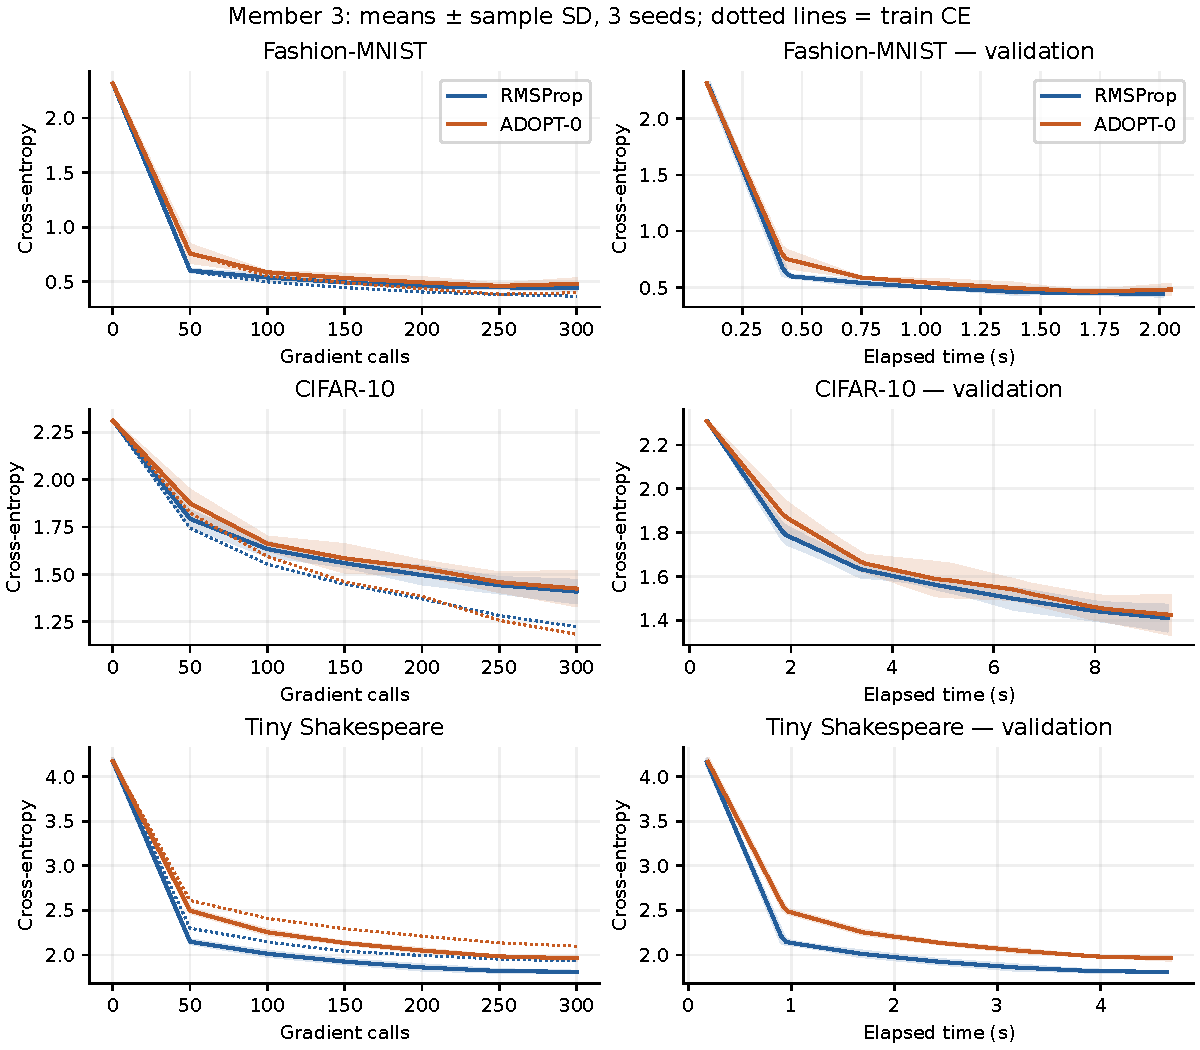
\includegraphics[width=.94\linewidth]{figures/member3_overview.pdf}
\caption{Member 3: solid curves show validation CE, dotted curves show mean training CE;
bands are $\pm1$ sample SD across three seeds. Left: gradient calls. Right: validation CE
interpolated onto a common time grid within each optimizer's observed interval.
Evaluation uses the fixed prefixes described in Setup.}\label{fig:m3-overview}
\end{figure}

\paragraph{Stability and cost.}
Both methods first pass the predeclared validation thresholds (1.0/2.0/3.0) at call 50
in every seed. This coarse metric cannot distinguish their early progress.
ADOPT-0 is approximately 1.0--1.1\% slower here; such small single-machine timing differences
are not a robust efficiency ranking. Both store 437,544 / 102,312 / 100,484 bytes of optimizer
state tensors on Fashion / CIFAR / Text. There are no observed failures, but only three main
seeds and 300 calls; this does not establish general numerical stability.
\FloatBarrier
